\documentclass[aspectratio=169,11pt]{beamer}
\usepackage[T1]{fontenc}
\usepackage{lmodern}
\usepackage{booktabs}
\usepackage{tikz}
\usetikzlibrary{arrows.meta,positioning}
\usepackage{pgfpages}   % needed for the notes layout below

% SPEAKER NOTES. This one line puts each slide on the left half of the PDF page and its
% \note{...} on the right half, which is what Lemmata's presenter view shows (slide for the
% audience, notes for you). To share or print plain slides, delete or comment out this line:
% the \note commands are then ignored and every page is just a slide.
\setbeameroption{show notes on second screen=right}
% The notes half: plain text on a pale page, large enough to read at a glance.
\setbeamertemplate{note page}{\pagecolor{yellow!8}\insertnote}
\setbeamerfont{note page}{size=\Large}

% A clean built-in look: slide title in a bar, author and page number in the footline.
\usetheme{Boadilla}
\usecolortheme{whale}
\setbeamertemplate{navigation symbols}{}
\setbeamertemplate{itemize items}[circle]

\title{Title of the Talk}
\subtitle{One line that says what the audience will take home}
\author{Your Name}
\institute{Institution}
\date{Conference or Seminar, \today}

\begin{document}

\begin{frame}[plain]
  \titlepage
  % A note can sit inside the frame it belongs to, anywhere in it.
  \note{Greet the audience, say who you are and how long you will talk. Open with the one
    sentence you want them to remember, not with an outline.}
\end{frame}

\begin{frame}{The problem in one slide}
  \begin{itemize}
    \item One idea per slide; say the rest aloud.
    \item At most four bullets of a line each.
    \item End the slide on its message, not on a list.
  \end{itemize}
  \note{
    \begin{itemize}
      \item Tell the story behind the problem here: the example that made you care.
      \item Ask the audience a question if the room is small.
      \item Time check: about two minutes so far.
    \end{itemize}
  }
\end{frame}

\begin{frame}{Approach}
  \begin{columns}[T]
    \begin{column}{0.5\textwidth}
      A diagram explains faster than prose:
      \begin{itemize}
        \item data goes in
        \item the model learns
        \item results come out
      \end{itemize}
    \end{column}
    \begin{column}{0.5\textwidth}
      \centering
      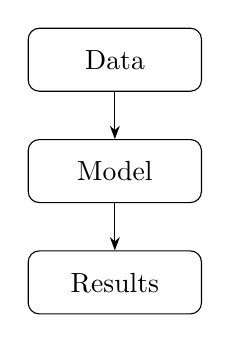
\begin{tikzpicture}[node distance=6mm, box/.style={draw, rounded corners, minimum width=22mm, minimum height=8mm}]
        \node[box] (a) {Data};
        \node[box, below=of a] (b) {Model};
        \node[box, below=of b] (c) {Results};
        \draw[-{Stealth}] (a) -- (b);
        \draw[-{Stealth}] (b) -- (c);
      \end{tikzpicture}
    \end{column}
  \end{columns}
  \note{Walk through the diagram top to bottom, one box per sentence. Point out what is new
    compared with the usual pipeline. Do not read the bullets.}
\end{frame}

\begin{frame}{Results}
  \centering
  \begin{tabular}{@{}lrr@{}}
    \toprule
    Method & Accuracy (\%) & Time (s) \\
    \midrule
    Baseline & 81.2 & 12 \\
    Ours & \textbf{86.9} & 15 \\
    \bottomrule
  \end{tabular}
  \note{State the one number that matters (5.7 points better) before the audience reads the
    table. Mention the 3-second cost honestly. Be ready for the question about variance:
    five runs, standard deviation 0.4.}
\end{frame}

\begin{frame}{Takeaways}
  \begin{enumerate}
    \item The one thing you want them to remember.
    \item The second thing.
    \item What to try next, or where to find the code.
  \end{enumerate}
  \note{Repeat the main message in the words of the first slide. Thank the audience and the
    co-authors, then invite questions. Backup slides, if any, go after this frame.}
\end{frame}

\end{document}
